
\chapter{Arquitetura de Software}
\label{sec-arquitetura}
\vspace{-1cm}

A Figura~\ref{figura-arquitetura} mostra a arquitetura do sistema \emph{\imprimirtitulo}.

\begin{figure}[h]
	\centering
	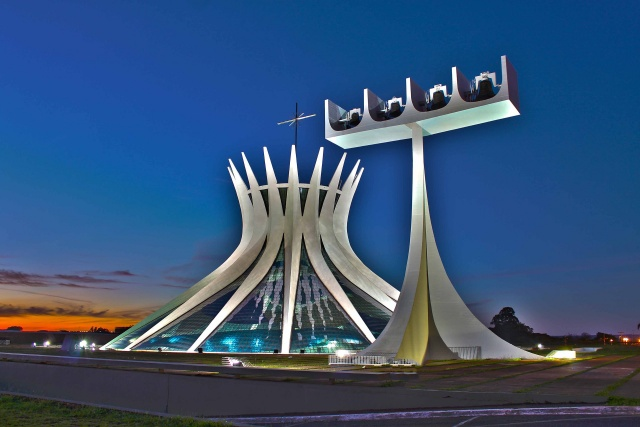
\includegraphics[width=0.8\textwidth]{figuras/figura-arquitetura}
	\caption{Arquitetura do sistema.}
	\label{figura-arquitetura}
\end{figure}

\vitor{Substituir a Figura~\ref{figura-arquitetura} pelo diagrama UML da arquitetura do seu projeto e descrevê-la no texto. Caso use alguma arquitetura clássica, incluir referência bibliográfica com BibTeX (ex.:Camada de Serviço~\cite{fowler:book02}). Como exemplo, vide documentos de projeto do Marvin e da Locadora de Carros do prof. Ricardo Falbo.}

\vspace{0.5cm}

A arquitetura do sistema \emph{\imprimirtitulo} é baseada em uma combinação dos estilos em camadas e partições. Ela é composta por dois principais subsistemas, organizados em três camadas.
\begin{itemize}
	\item \textbf{Subsistema Controle Interno:} Responsável pelo gerenciamento interno do sistema, incluindo cadastro e manutenção de dados de funcionários, produtos, serviços e filiais.
	\item \textbf{Subsistema Atendimento Cliente:} Responsável pela interação com os clientes, abrangendo cadastro e login de clientes, agendamentos de serviços, histórico de atendimentos e registro de compras.
\end{itemize}
As camadas da arquitetura de cada subsistema são definidas como:
\begin{itemize}
	\item \textbf{Camada de Interface com o Usuário (CIU):} Responsável pela comunicação entre o usuário e o sistema, incluindo telas e controladores de interação.
	\item \textbf{Camada de Lógica de Negócio (CLN):} Implementa a lógica de aplicação e de domínio do problema. Aplica-se o padrão Camada de Serviço (Service Layer), separando a lógica de tarefas (CGT) da lógica de domínio (CDP).
	\item \textbf{Camada de Gerência de Dados (CGD):} Responsável pela persistência e recuperação de dados, seguindo o padrão Data Access Object (DAO).
\end{itemize}
A comunicação entre as camadas segue o padrão MVC, onde as classes controladoras de interação (CIU) interagem com as classes gerenciadoras de tarefas (CGT), que por sua vez se comunicam com as classes do domínio do problema (CDP) e com as classes de acesso a dados (CGD).

\vspace{0.5cm}
